\documentclass[12pt]{article}

\usepackage{graphicx}
\usepackage{html}
\usepackage{amssymb}
\usepackage{hyperref}

\renewcommand{\familydefault}{\sfdefault}

\setlength{\textwidth} {6.5 true in}
\setlength{\textheight}{9 true in}
\setlength{\hoffset}   {-0.50 true in}
\setlength{\voffset}   {-0.75 true in}

\begin{document}

\begin{latexonly}
\subsection*{Calculating Determinants}
\end{latexonly}

\begin{itemize}
\item The determinant of a $2 \times 2$ matrix

  \begin{equation}
M = 
\left(
\begin{array}{cccc}
m_{11}  & m_{12} \\
m_{21}  & m_{22} 
\end{array}
\right)
\end{equation}

\noindent
is given by

\begin{equation}
|M| = 
\left|
\begin{array}{cccc}
m_{11}  & m_{12} \\
m_{21}  & m_{22} 
\end{array}
\right|
= m_{11} \, m_{22} - m_{12} \, m_{21}
\end{equation}

\item The determinant of a $3 \times 3$ matrix

\begin{equation}
M =
\left(
\begin{array}{cccc}
m_{11}  & m_{12} & m_{13} \\
m_{21}  & m_{22} & m_{23} \\
m_{31}  & m_{32} & m_{33} 
\end{array}
\right)
\end{equation}

\noindent
can be written in terms of the determinants of $2 \times 2$
sub-matrices 

\begin{equation}
|M| =
\left|
\begin{array}{cccc}
m_{11}  & m_{12} & m_{13} \\
m_{21}  & m_{22} & m_{23} \\
m_{31}  & m_{32} & m_{33} 
\end{array}
\right| \\
= m_{11} 
\left|
\begin{array}{cccc}
m_{22}  & m_{23} \\
m_{32}  & m_{33} 
\end{array}
\right| 
\,-\, m_{12} 
\left|
\begin{array}{cccc}
m_{21}  & m_{23} \\
m_{31}  & m_{33} 
\end{array}
\right| 
\,+\, m_{13} 
\left|
\begin{array}{cccc}
m_{21}  & m_{22} \\
m_{31}  & m_{32} 
\end{array}
\right|
\end{equation}

\item In general, each element of the top row of the matrix is
  multiplied by the determinant of the sub-matrix obtained by removing
  the row and column containing that element. The results are
  then added together with alternating sign, starting with a positive
  $m_{11}$ term. Figure~1 %\ref{fig:dets}
  shows the top-row elements and the associated sub-matrices and signs
  for the $2 \times 2$, $3 \times 3$, and $4 \times 4$ cases.

\end{itemize}

%\begin{figure}[h!]
\begin{center}
%\scalebox{0.6}{
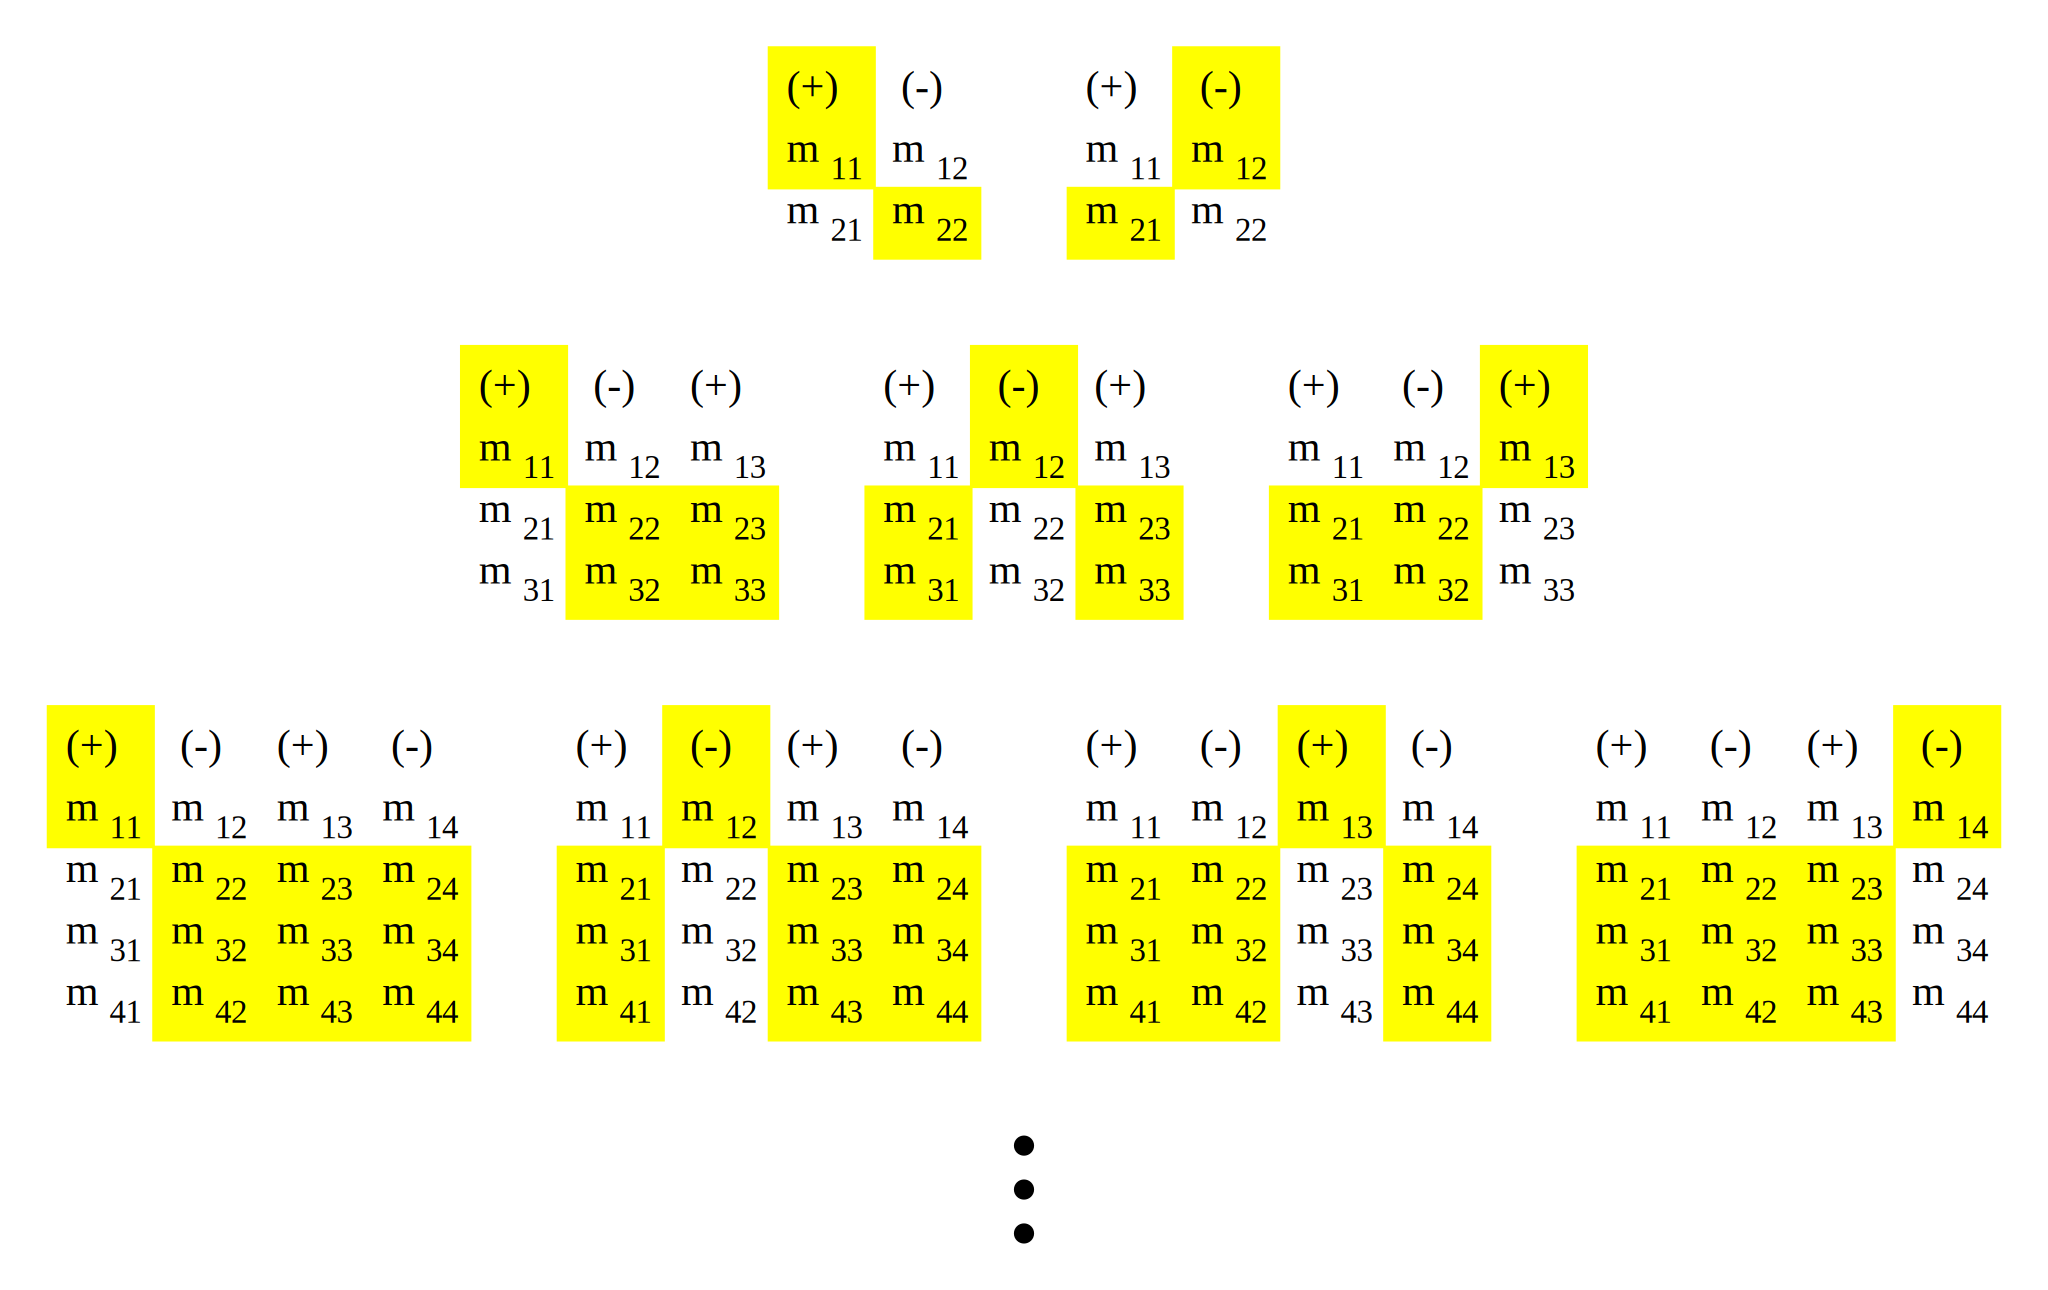
\includegraphics{dets.png}
%}

Figure 1: A visual guide to computing the determinants of $2 \times 2$,
$3 \times 3$, and $4 \times 4$ matrices.

%\caption{A visual guide to computing the determinants of $2 \times 2$, $3
%  \times 3$, and $4 \times 4$ matrices.}
%\label{fig:dets}
\end{center}
%\end{figure}

\subsubsection*{An $\mathbf{n=2}$ Example}

\begin{equation}
M =  
\left(
\begin{array}{cccc}
3  & -1 \\
5  &  7 
\end{array}
\right)
\end{equation}

\begin{equation}
|M| = 3 \cdot 7 - (-1)\cdot 5 = 21 + 5 = 26
\end{equation}

\subsubsection*{An $\mathbf{n=3}$ Example}

\begin{equation}
M =
\left(
\begin{array}{cccc}
 4 &  2 & 5 \\
-1 &  6 & 7 \\
 3 &  1 & 2
\end{array}
\right)
\end{equation}

\begin{equation}
|M| =
4
\left|
\begin{array}{cccc}
6 & 7 \\
1 & 2
\end{array}
\right| 
\,-\, 2
\left|
\begin{array}{cccc}
-1 & 7 \\
 3 & 2
\end{array}
\right| 
\,+\, 5
\left|
\begin{array}{cccc}
-1 & 6 \\
 3 & 1
\end{array}
\right|
\end{equation}

\begin{equation}
= 4 \, (6 \cdot 2 - 7 \cdot 1)
  - 2 \, ((-1) \cdot 2 - 7 \cdot 3)
  + 5 \, ((-1) \cdot 1 - 6 \cdot 3)\\
= 20 + 46 - 95 \\
= -29
\end{equation}

{\footnotesize
  \noindent
  \hrulefill
  
  \noindent
  This work is licensed under the Creative Commons
  Attribution-ShareAlike 4.0 International License: 
  \url{http://creativecommons.org/licenses/by-sa/4.0/}.\\

  \noindent
  L.A. Riley (\texttt{lriley@ursinus.edu}), updated June 2021
}

\end{document}
